\documentclass[a4paper, 11pt, oneside, openright, english]{book}
\usepackage[utf8]{inputenc}
\usepackage{graphicx}
\usepackage{hyperref}
\usepackage{booktabs}
\usepackage{blindtext}
\usepackage{amsmath}
\usepackage{amssymb}
\usepackage{listings}
\usepackage{titlesec}
% \usepackage{xcolor}
\usepackage{longtable}
\usepackage{seqsplit}
\usepackage{geometry}
\usepackage{fancyhdr}
\usepackage{float}
\usepackage{enumitem}
\usepackage{array}
\usepackage{multicol}
\usepackage{caption}
\usepackage{listings}
\usepackage[T1]{fontenc}  % Use T1 font encoding
\usepackage{beramono}
\usepackage[dvipsnames]{xcolor}


\pagestyle{fancy}
\fancyhf{}

\fancyhead[LE,RO]{\slshape \rightmark}
\fancyhead[LO,RE]{\slshape \leftmark}
\fancyfoot[C]{\thepage}
\renewcommand{\chaptermark}[1]{\markboth{#1}{}}
\renewcommand{\sectionmark}[1]{\markright{\thesection.\ #1}}

\setlength{\headheight}{13.59999pt}
\addtolength{\topmargin}{-1.59999pt}

\titleformat{\chapter}[block]{\normalfont\huge\bfseries}{\thechapter.}{1em}{\Huge}

\begin{document}

\begin{titlepage}
    \begin{center}
        
\includegraphics[width=0.8\textwidth]{../images/PoliMi_Logo.png}

        \vspace*{2cm}
        \textbf{\huge Image Analysis and Computer Vision}

        \vspace{0.5cm}
        \LARGE Homework 

        \vspace{1.5cm}
        \normalsize IACV homework\\
        Academic year 2023 \- 2024


        \vspace{1cm}
        \small
        \begin{table}[b]
            \centering
            \begin{tabular}{l p{5.5cm} l}
                \textit{Author:}   &  \\
                Michelangelo Stasi  & 
            \end{tabular}
        \end{table}

    \end{center}
\end{titlepage}

\tableofcontents
\chapter{Introduction}
In this project, from an image we have to extract features and calculate parameters important for the analysis of the image.\\
The project is divided in two parts : 
\begin{itemize}
    \item \textbf{Theory} : in this part we will solve theoretical problems with parameters starting from the image given, using projective and camera geometry. (Figure \ref{fig:contours})
    \item \textbf{MatLab} : in this part we have to implement through MatLab scripts the solutions given in the first part
\end{itemize}
\begin{figure}[H]
    \centering
    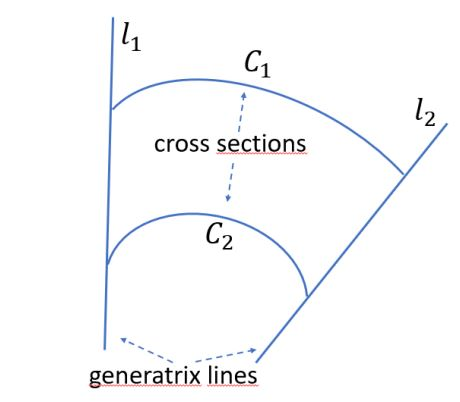
\includegraphics[width=0.3\textwidth]{../images/contours.JPG}
    \caption{Contours of the cylinder assigned.}
    \label{fig:contours}    
\end{figure}
The scene has different parallel elements, such as \textbf{$l_1$ and $l_2$}, which can be useful to compute features of the image.\\
The tricky part will be the computation of the calibration matrix \textbf{$K$}, since the camera used can not be assumed to be natural : 
therefore, the matrix $K$ wil have \textbf{four unknowns}.\\
It is assumed that the parameters of \textbf{$C_1$, $C_2$, $l_1$, $l_2$} have been exctracted a priori.\\
\chapter{Theory}
\section{Problem 1}
\textbf{From \textit{C1},\textit{C2} find the horizon(vanishing) line \textit{$h$} of the plane orthogonal to the cylinder axis.}\\
One of the assumptions is the knowledge of the geometrical properties of $C_1$,$C_2$, which are conics defined by the following equations : \\
\begin{equation}
    C1 : a1X^2 + b1XY + c1Y^2 + d1X + e1Y + f1 = 0
\end{equation}
\begin{equation}
    C2 : a2X^2 + b2XY + c2Y^2 + d2X + e2Y + f2 = 0
\end{equation}
They can also be defined in matrix form : \\
\begin{equation}
    x^TCx = 0 \\
\end{equation}

\[
    C_i = 
\begin{pmatrix}
    a_i & b_i/2 & d_i/2 \\
    b_i/2 & c_i & e_i/2 \\
    d_i/2 & e_i/2 & f_i 
\end{pmatrix}
\]
\[
    x = 
\begin{pmatrix}
    X \\
    Y \\
    1
\end{pmatrix}
\]
Where i = 1,2.\\
\\From the theory, the intersection between $C_1$ and $C_2$ is the image of the circular points. \\
\begin{equation}
        C1 \cap  C2 = \{ I', J'\} \label{eq:IJ}
\end{equation}
The circular points by definition are points at the infinity. \\
\[
    I =  
\begin{pmatrix}
    1 \\
    i \\
    0
\end{pmatrix}    
\]
\[
    J =  
\begin{pmatrix}
    1 \\
    -i \\
    0
\end{pmatrix}    
\]
The line at the infinity is the locus of the points at the infinity and 
in order to calculate it we have to find the equation of the line passing through the circular points :
\begin{equation}
    l'_\infty = I' \times J' 
\end{equation}    
The line we have found is \textbf{h}, the horizon stated in the problem text, since the plane we are considering is orthogonal to the cylinder axis.


\section{Problem 2}
\textbf{From \textit{l1}, \textit{l2}, \textit{C1}, \textit{C2} find the image projection \textit{a} of the cylinder axis, and its vanishing point V.}\\
Since \textit{l1} and \textit{l2} are both generatrix lines, by definition they are parallel to the cylinder's axis.\\
As a conclusion, the vanishing point of \textit{$l_1$} and \textit{$l_2$} will be the vanishing point $V$ mentioned in the text (Figure \ref{fig:vanishinpoint}).\\
\begin{equation}
    V = l1 \cap l2 \label{eq:V}
\end{equation}

\begin{figure}[H]
    \centering
    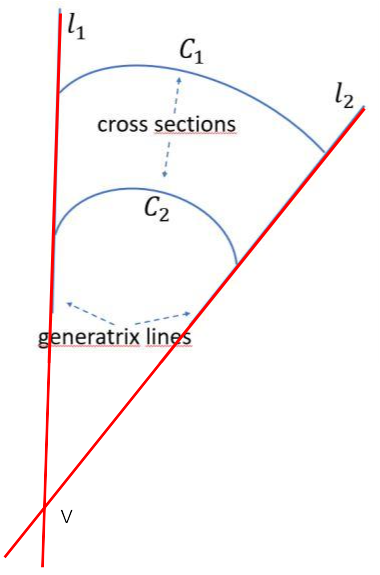
\includegraphics[width=0.3\textwidth]{../images/vanishinpoint.png}
    \caption{ Intersection of \textit{l1 l2} at the vanishing point V.}
    \label{fig:vanishinpoint}
\end{figure}
In order to find the axis of the cylinder, firstly we have to compute the centers of the circular cross sections.\\
From the theory, the polar line of a point at the infinity, with respect to a circumference, is the diameter orthogonal to the direction of the point.\\
Polarity is preserved under projective mapping, then diameters will map onto diameter ;\\ since we have two images of points at the infinity (\textbf{$I'$ and $J'$}), therefore we can find the images of the diamaters.
\begin{equation}
    d1 = C1 * I';
\end{equation}
\begin{equation}
    d2 = C1 * J';
\end{equation}
\begin{equation}
    d3 = C2 * I';
\end{equation}
\begin{equation}
    d4 = C2 * J';
\end{equation}
The centers \textbf{$O_1$, $O_2$} can be derived as the intersections of, respectively, \textbf{$d_1$ with $d_2$} and \textbf{$d_3$ with $d_4$} :  
\begin{equation}
    O1 = d1 \cap d2
\end{equation}
\begin{equation}
    O2 = d3 \cap d4
\end{equation}
Therefore, \textit{a} is the line passing through the centers \textit{$O_1$, $O_2$} :
\begin{equation}
    a = O_1 \times O_2
\end{equation}

\section{Problem 3}
\textbf{From \textit{l1, l2, C1, C2} (and possibly \textit{h, a}, and \textit{V}), find the calibration matrix \textit{K}.}\\ 
From the thory, the calibration matrix \textit{K} is :
\[
    K = 
\begin{pmatrix}
    f_x & s   & U_0 \\
    0   & f_y & V_0 \\
    0   & 0   & 1
\end{pmatrix}    
\] 
Since the camera is with zero-skew (this is given by the text), \textit{s = 0}.\\
Therefore we have \textbf{four unknowns}, because the camera is \textbf{not natural} and as a consequence : \[ f_x \neq f_y\]
The camera principal point ($U_0, V_0$) is the projection of the camera center onto image plane.\\
From the theory we know that the absolute conic is defined as follow : 
\[
    \varOmega_\infty =  
\begin{pmatrix}
    1 & 0 & 0 \\
    0 & 1 & 0 \\ 
    0 & 0 & 1
\end{pmatrix}    
\]
The transformation depends only on intrinsics camera parameters. Therefore the image of the absolute conic IAC is given by : 
\begin{equation}
    IAC = \omega = M^{-T} \varOmega M^{-1} = K^{-T}R^{-T}\varOmega_\infty K^{-1}R^{-1} = K^{-T}K^{-1} \label{eq:omega}
\end{equation} 
As a consequence the DIAC is given by : 
\begin{equation}
    DIAC = \varOmega^{*} = KK^{T}
\end{equation}
Therefore we can use Cholesky Factorization to get the matrix K.\\
The only problem is to get the image of the absolute conic (IAC).\\
We can use orthogonal lines and their vanishing points to retrieve two equations.\\
A pair of orthogonal lines could be \textbf{$d_1$ and $d_2$} (computed in the first problem through $C_1$ and $C_2$), since they are diamaters orthogonal to directions x and y, which are orthogonal.\\
We have to find two vanishing points, and to do this we will use \textbf{$d_3$ and $d_4$}, the diamaters of the conic $C_2$, since they are parallel to, respectively, $d_1$ and $d_2$.
\begin{equation}
    v1 = d1 \cap d3 \label{eq:v1}
\end{equation}
\begin{equation}
    v2 = d2 \cap d4 \label{eq:v2}
\end{equation}
Since the vanishing point \textbf{V} is obtained with parallel lines which are generatrices of the cylinder, then they are orthogonal to all diamaters.\\
Therefore we can exploit orthogonality by calculating the cosine of the angle between the directions of the lines.
\begin{equation}
    \cos(\theta) = \frac{d_1^{T}d_2}{\sqrt[]{(d_1^{T}d_1)(d_2^{T}d_2)}} = \frac{v_1^{T}\omega v_2}{\sqrt[]{(v_1^{T}\omega v_1)(v_2^{T}\omega v_2)}} 
\end{equation}
Where, only in this equation, $d_1$ and $d_2$ are directions of two generic lines, $v_1$ and $v_2$ are their vanishing points and theta is the angle between the directions $d_1$ and $d_2$.\\
The equations obtained are :
\begin{equation}
    \cos(\theta) = 0 = v_1^{T}\omega v_2
\end{equation}
\begin{equation}
    \cos(\theta) = 0 = V^{T}\omega v_1
\end{equation}
Where $v_1$ and $v_2$ are the vanishing points computed in the equations \ref{eq:v1} and \ref{eq:v2}, $\omega$ is retrieved from the equation \ref{eq:omega} and V is the vanishing point computed in the equation \ref{eq:V}.
\\The following equations are derived from circular points of the conics \textit{C1 and C2}. \\
Since by definition the image of absolute conic contains the image of all circular points, IAC has to satisfy these equations :
\begin{equation}
    I'^{T}\omega I' = 0
\end{equation}
\begin{equation}
    J'^{T}\omega J' = 0
\end{equation}
By solving these four equations we will find the IAC and as a consequence we can also compute the DIAC to finally get the calibration matrix through Cholesky Factorization.


\section{Problem 4}
\textbf{From \textit{h}, \textit{K}, and \textit{V} determine the orientation of the cylinder axis wrt the camera reference.}\\
Our image plane contains the line at the infinity \textbf{h}.\\
The camera has zero-skew property, which means that lines at the infinity converge to the image center.\\
Then the image plane is parallel to the principal plane of the camera, which is the plane containing the optical center and the principal point.\\
Then, the angle that the direction of the line at the infinity makes defines the orientation of the cylinder axis wrt the camera' reference .
\\The  angle can be determined as :
\begin{equation}
    \theta = \cos ^{-1}(\rho )
\end{equation}
Where : 
\begin{equation}
    \rho  = \cos(\theta) = \frac{h^{T}a}{\sqrt[]{(h^{T}h)(a^{T}a)}}
\end{equation}
\section{Problem 5}

\textbf{Compute the ratio between the radius of the circular cross sections and their distance.}\\
We have to make an affine rectification and map the section between the circular cross sections to a parallelogram.\\
We can do this by finding a matrix \textbf{$H_{\text{R}}$} such that multipied by an image point, it gives back the rectified point.\\
We can use \textbf{$H_{\text{R}}$} to find the rectified circular cross sections and then measure their diameters and their distances.\\
In fact from the theory, the ratio of the diameter and the distance between the two circular cross sections is preserved under rectification: 
\begin{equation}
    d/D 
\end{equation}
Note that the diameter \textbf{d} is equal to \textbf{2*r},
where \textbf{r} is the radius of the circual cross section.\\
From the theory we know that the dual absolute conic is given by : 
\begin{equation}
    C_\infty^{*} = IJ^{T} + JI^{T}
\end{equation}
and its image is :
\begin{equation}
    C_\infty'^{*} = I'J'^{T} + J'I'^{T}
\end{equation}
which we can compute since we know both \textbf{$I'$} and \textbf{$J'$} obtained from \ref{eq:IJ}.\\
The dual absolute conic \textbf{$C_\infty^*$} is also obtained from a transformation over \textbf{$C_\infty^*$}. In fact, from the theory :
\begin{equation}
    C_\infty^* = H_R C_\infty'^* H_R^{T}
\end{equation}   
and therefore : 
\begin{equation}
    C_\infty'^* = H_R^{-1} C_\infty* H_R^{-T}
\end{equation}
Since we know how \textbf{$C_\infty^*$} is mapped, we can find \textbf{$H_{\text{R}}$} using the singular value decomposition, which for a generic matrix M it returns : 
\begin{equation}
    SVD(M) = USV^T
\end{equation}
If M is symmetric, $U = V$. Since \textbf{$C_\infty^*$} is symmetric : 
\begin{equation}
    SVD(C_\infty'^*) = H_R^{-1} C_\infty H_R^{-T} = USU^T
\end{equation}
Therefore $H_R = U^{-1}$ and by finding two pairs of diametrically opposed points on the conics and by getting the rectified points $\tilde{x} _i = H_R x_i'$ we can compute the ratio with the new rectified points.\\
In fact, in an affinely rectified image, the ratio of parallel lenghts is preserved.



\chapter{MatLab}
\section{Preprocessing}
\textbf{The code is in main.m file.}\\
Since the second conic $C_2$ is difficult to distinguish from the surface of the cylinder, 
it has been applied an effective edge detection filter on the gray scaled image.\\
There are different types of edge detection filter, but the \textit{'Canny'} filter is the most effective on this image.\\
The result of the preprocessing is shown in figure \ref{fig:preproccesing}
\begin{figure}[H]
    \centering
    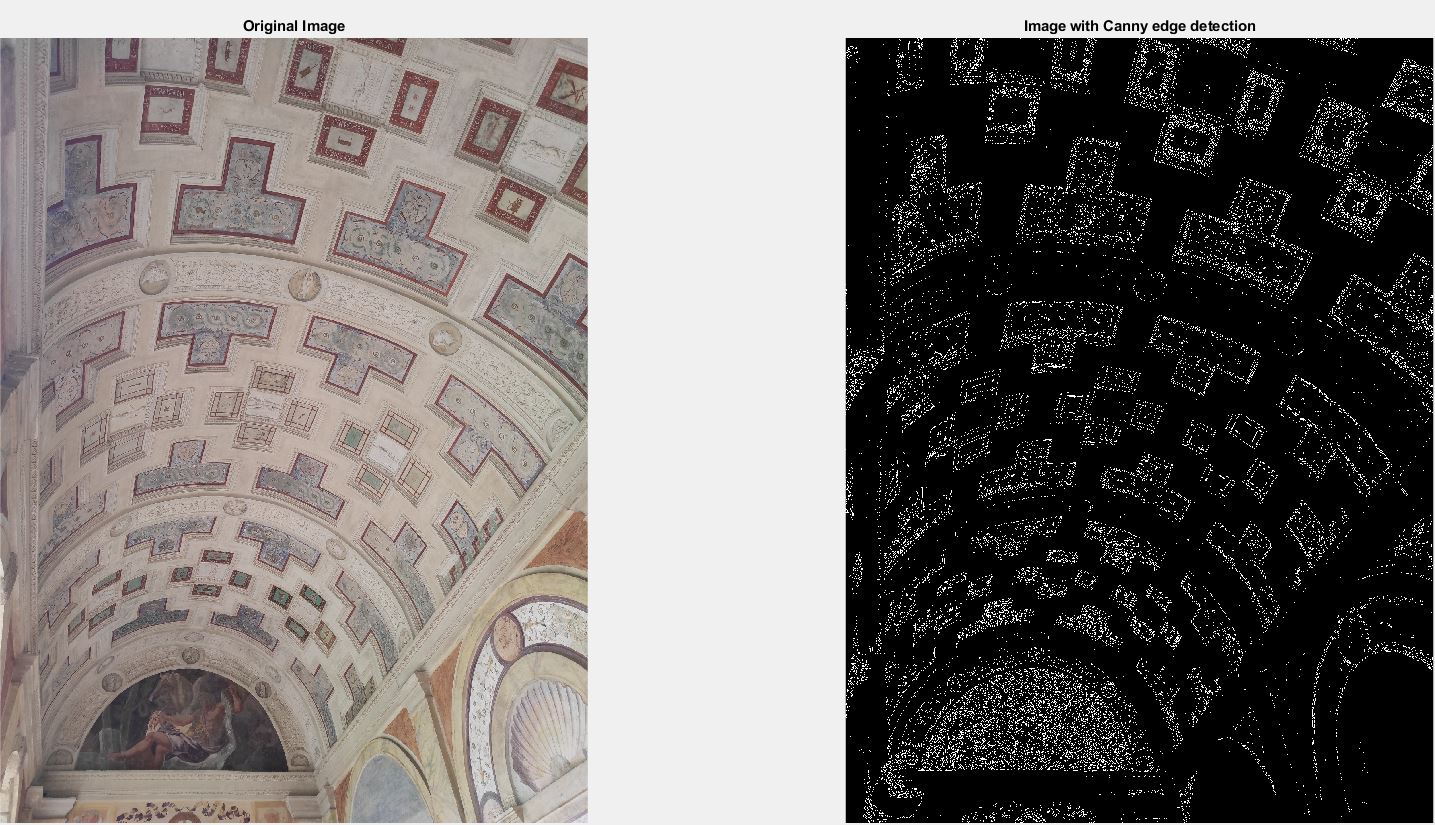
\includegraphics[width=\textwidth]{../images/preprocessing.JPG}
    \caption{ Original image and preprocessed image with \textit{'Canny'} filter.}
    \label{fig:preproccesing}
\end{figure}
\section{Features Extraction}
\textbf{The code is in main.m file.}\\
From the preprocessed image, I selected six points for each conic to find.\\
For the conic $C_1$ and $C_2$ I selected the following points : 
\begin{figure}[H]
    \centering
    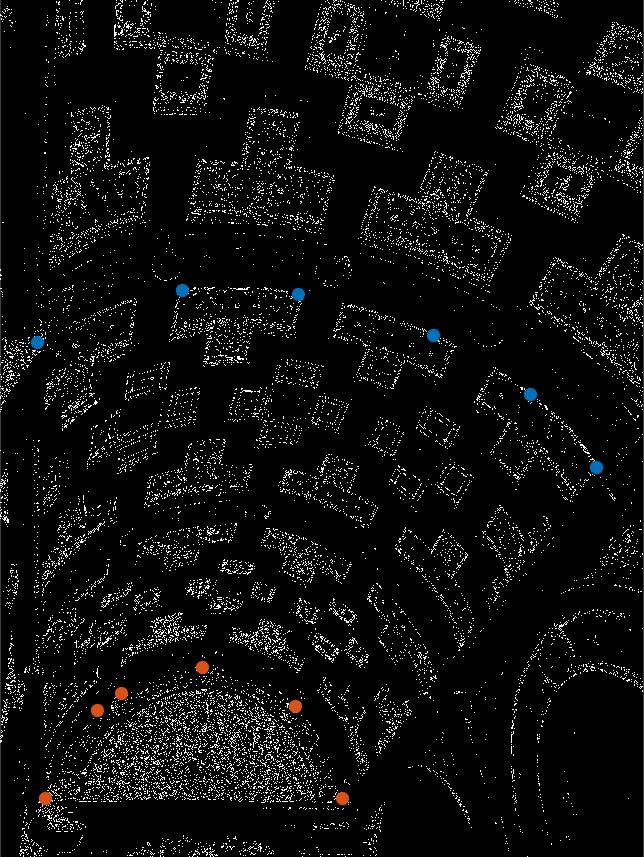
\includegraphics[width=0.7\textwidth]{../images/pointsSelected.JPG}
    \caption{Points selected for the first and second conic.}
\end{figure}

The orange points are the ones for the conic $C_2$, whereas the blue points are the ones for the conic $C_1$.\\
Notice how, despite the use of the Canny filter, the edges of the second conic are not really visible, so it has been used the contour of the paint.\\
The resulting images of generatrix lines $l_1$ and $l_2$ and of circular cross sections $C_1$ and $C_2$ are the following:

\begin{figure}[H]
    \centering
    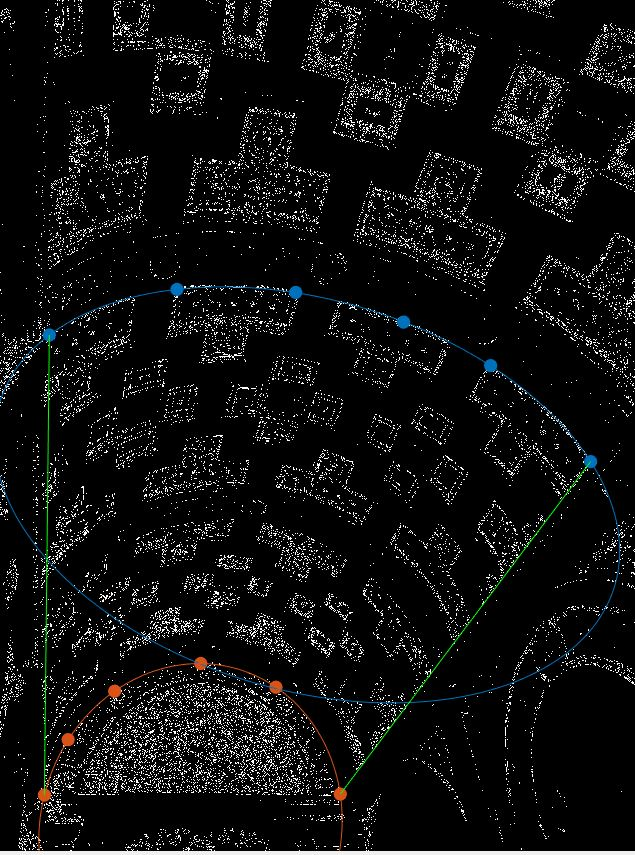
\includegraphics[width=0.7\textwidth]{../images/images.JPG}
    \caption{Images of features.}
\end{figure}
The images of the horizon line $h$ and the axis of the cylinder $a$ is the following : 
\begin{figure}[H]
    \centering
    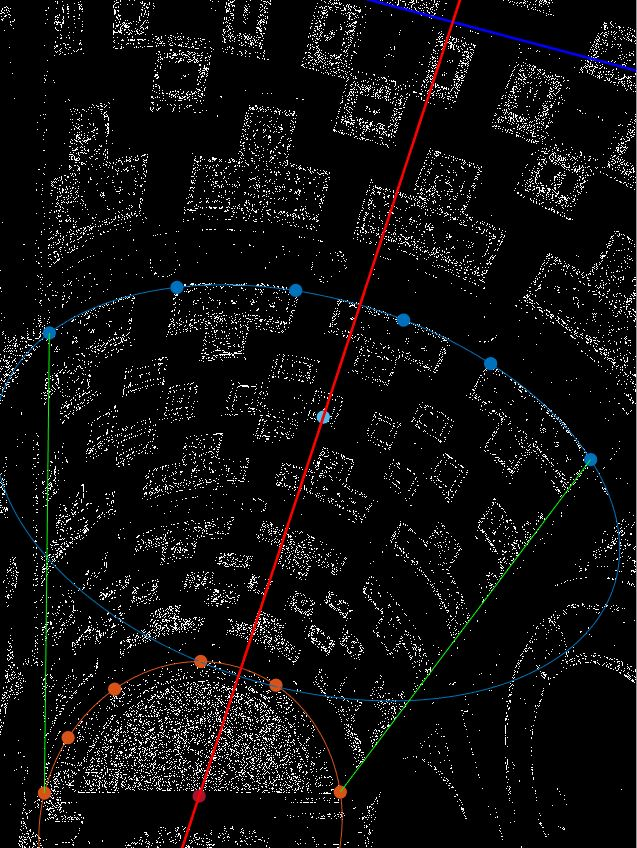
\includegraphics[width=0.7\textwidth]{../images/features.JPG}
    \caption{Images of horizon (blue line) and cylinder axis (red line).}
\end{figure}
Note that the axis and the horizon line strictly depend on which point you have chosen for the computation of $C_1$ and $C_2$.\\
The parameters of the resulting calibration matrix $K$ are the following : 
\[
    K = 1.0e+04* 
\begin{pmatrix}
    0.5577 & 0 & 4.56\\
    0  & 1.4164& 1.35 \\
    0  &  0  & 0.001 \\
\end{pmatrix} 
\]
\begin{equation}
    a = 0.39
\end{equation}
where $a$ is the aspect ratio.\\
The orientation of the cylinder axis wrt the camera reference is given by the angle between the axis $a$ and the horizon line $h$ : \\
\begin{equation}
    angle = 89.9
\end{equation}
\section{Rectification of a cylindric surface}
\textbf{The code is in rect.m file.}\\
The method used is the affine reconstruction. I have selected four points such that the lines passing through them 
are reciprocally orthogonal : in fact, $\overline{AB} \perp \overline{CD} $ and $\overline{AC} \perp \overline{BD}$. 
\begin{figure}[H]
    \centering
    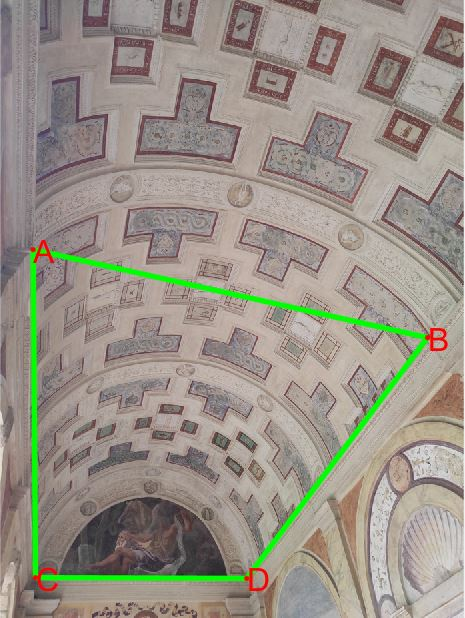
\includegraphics[width=0.7\textwidth]{../images/section.JPG}
    \caption{Section selected.}
\end{figure}
Then I computed the vanishing points and the vanishing line of that plane : therefore, I can compute the rectification matrix $H_R$:
\[
    H_R = 
\begin{pmatrix}
    * & * & * \\
    * & * & * \\
    &l_\infty'^{T}
\end{pmatrix}    
\]
The image has been scaled due to crashes caused by the size of the image when using \textbf{imwarp()}.
The final outcome is : 
\begin{figure}[H]
    \centering
    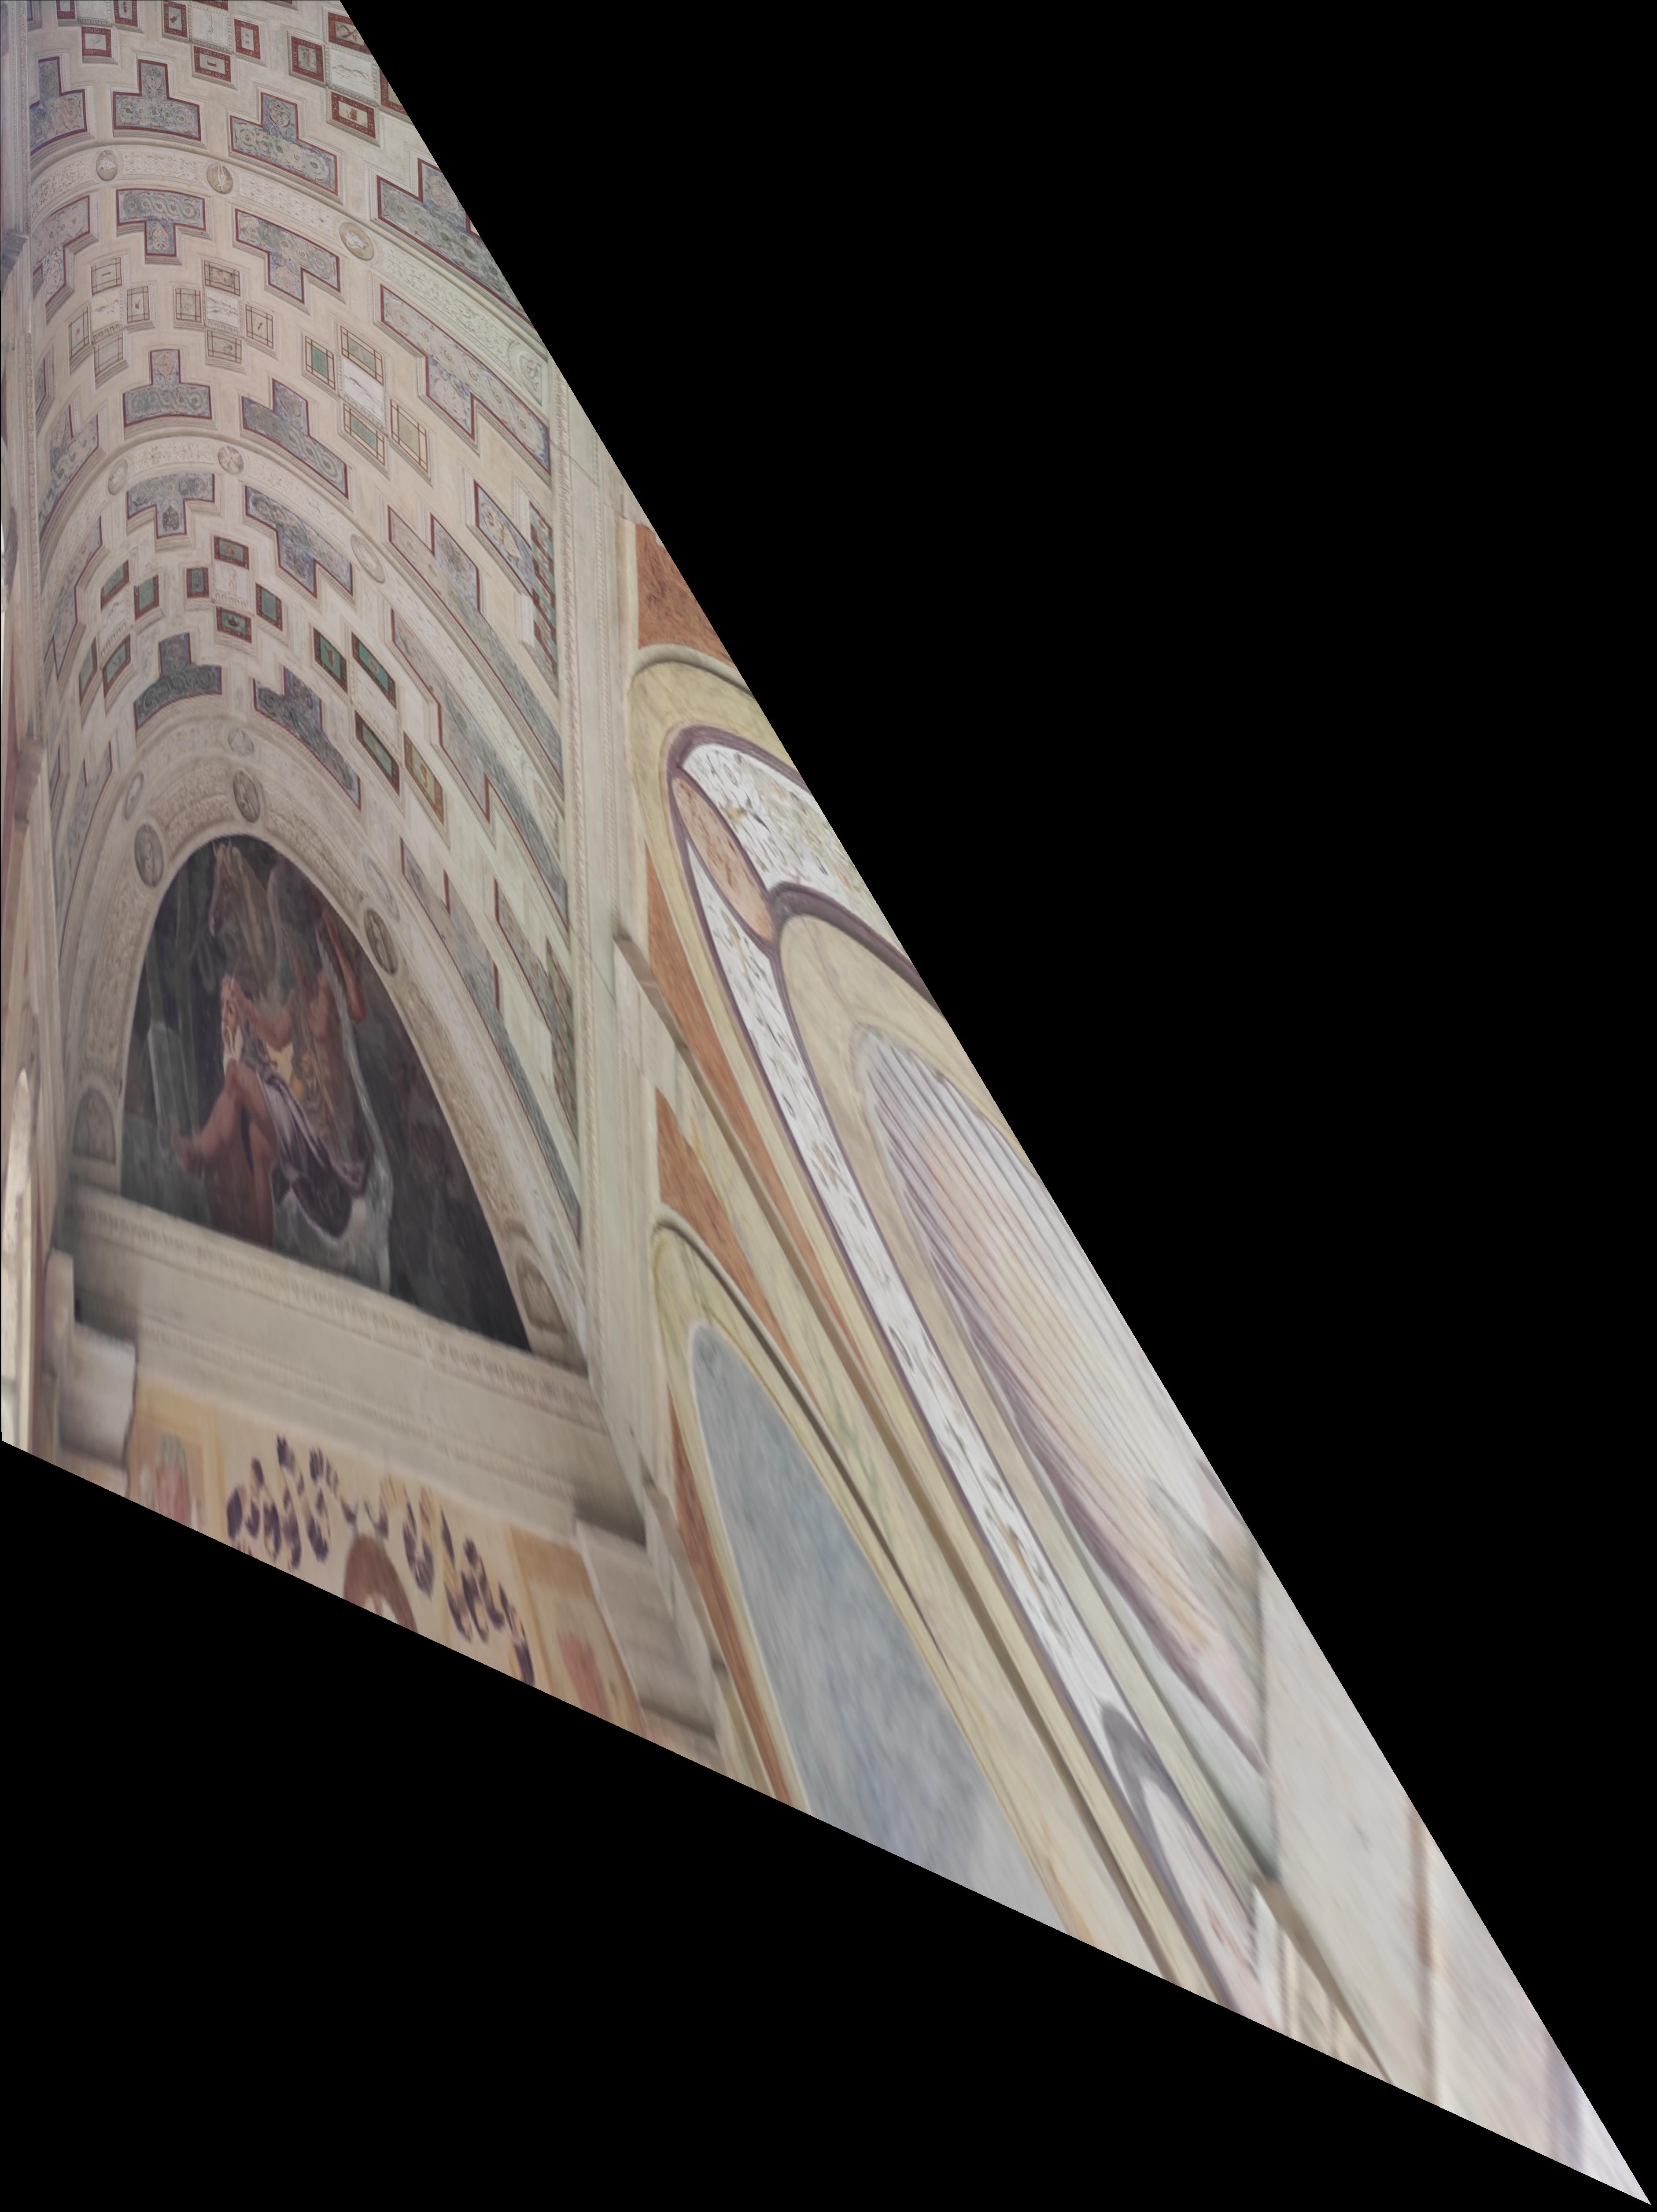
\includegraphics[width=0.7\textwidth]{../images/affRect.JPG}
    \caption{Rectified image.}
\end{figure}
\end{document}